\documentclass[11pt]{article}
\date{\vspace{-10ex}}

\usepackage{lineno,hyperref}
\modulolinenumbers[5]

%%%%%%%%%%%%%%%%%%%%%%%%%%%%%%%%%%%%%%%%%%%%%%%%%%%%%%%%%%%%%%%%%%%%%%%%%%
% Added lines by Gustavo Quintana to facilitate internal review process
\usepackage{amsmath, amsfonts, mathtools, hyperref, tikz, pgf, subcaption, mathdots}
\usepackage[a4paper, total={6.5in, 9in}]{geometry}
\usepackage{setspace}
\usetikzlibrary{shapes, arrows, calc, patterns, decorations.pathmorphing, decorations.markings, positioning, external}
\tikzexternalize
\tikzset{external/system call={pdflatex \tikzexternalcheckshellescape -halt-on-error -interaction=batchmode -jobname "\image" "\texsource" && pdftops -eps "\image.pdf"}}
\tikzexternalize[shell escape=-enable-write18]
\usepackage{algorithm, algorithmic, bm}
%\usepackage[noend]{algpseudocode}
\renewcommand{\algorithmicrequire}{\textbf{Input:}}
\renewcommand{\algorithmicensure}{\textbf{Output:}}
%\renewcommand{\algorithmicreturn}{\textbf{Initialize:}}

\makeatletter
\newcommand*\rel@kern[1]{\kern#1\dimexpr\macc@kerna}
\newcommand*\widebar[1]{%
  \begingroup
  \def\mathaccent##1##2{%
    \rel@kern{0.8}%
    \overline{\rel@kern{-0.8}\macc@nucleus\rel@kern{0.2}}%
    \rel@kern{-0.2}%
  }%
  \macc@depth\@ne
  \let\math@bgroup\@empty \let\math@egroup\macc@set@skewchar
  \mathsurround\z@ \frozen@everymath{\mathgroup\macc@group\relax}%
  \macc@set@skewchar\relax
  \let\mathaccentV\macc@nested@a
  \macc@nested@a\relax111{#1}%
  \endgroup
}
\makeatother
%%%%%%%%%%%%%%%%%%%%%%%%%%%%%%%%%%%%%%%%%%%%%%%%%%%%%%%%%%%%%%%%%%%%%%%%%%

%% `Elsevier LaTeX' style
\bibliographystyle{elsarticle-num}
%%%%%%%%%%%%%%%%%%%%%%%

\newtheorem{innercustomgeneric}{\customgenericname}
\providecommand{\customgenericname}{}
\newcommand{\newcustomtheorem}[2]{%
  \newenvironment{#1}[1]
  {%
   \renewcommand\customgenericname{#2}%
   \renewcommand\theinnercustomgeneric{##1}%
   \innercustomgeneric
  }
  {\endinnercustomgeneric}
}
\newcustomtheorem{customthm}{Theorem}
\newcustomtheorem{customlemma}{Lemma}

\DeclareMathAlphabet\mathbfcal{OMS}{cmsy}{b}{n}

\begin{document}


\title{Jury members' comments on the private PhD defense of \linebreak Gustavo Quintana-Carapia} 

\maketitle

Thank you to the jury members for reviewing the thesis manuscript and for giving suggestions for improvement. 
The manuscript changes due to the comments are highlighted in \color{blue} blue fontcolor\color{black}.

\section*{General comments}

\begin{itemize}
	\item The manuscript text should better position the PhD to related work. Improve the literature review and discuss (and cite) the state of the art.
	
	{\bfseries The introduction of the chapters now includes the state of the art to position the PhD work with respect to the literature.}
	
	\item  Add more clearly the motivation for the PhD research work by including motivational examples to the introduction.
	
	{\bfseries Motivational examples have been added to the Introduction. }
	
	\item  Add a discussion with comparison of existing EIV methods. Give, with the positive and negative aspects in mind, a better justification for why you use a (R)LS method, and not, e.g., (R)IV method.
	
	{\bfseries In Section 4.1.4, a discussion that compares IV methods with EIV methods has been added.}

	\item  Discuss more clearly the aspects of scalability of the methods and their limitations in terms of model order, size of data sets (e.g., related to the inversion of LS matrices).
	\item  The equations on pages 12 and 13 seemingly contain errors and should be corrected.
	
	{\bfseries The equations on pages 12 and 13 have been corrected.}
	
	\item  The figure shown on page 66 was made with a single experiment; it is desirable to see the (averaged) effect on several experiments.
	
	{\bfseries A series of 100 runs of the maximum-likelihod estimation method has been simulated and the results have been added to the manuscript in Section 6.3.2.}
	
\end{itemize}

\section*{Lyudmila Mihaylova}

\begin{itemize}
	\item You develop results for uncertainty quantification; what type of uncertainties  can your approach deal with and which levels of noise can you consider? Elaborate on SNR levels; I’m also very interested in scalability, so how big the matrices can be.
	\item  Concerning the scalability to data: eqn 3.6: how scalable is the approach in all aspects (order, data, linked to inversion for LS matrix); can you deal with hundreds, thousands of data?
	
	{\bfseries The following paragraph has been added in Section 3.2 to discuss the scalability of the data-driven step input estimation method.}
	
	\color{blue}
    The computational complexity of the RLS algorithm solution to the system of equations (3.14) is $O \left( \left( n+1 \right)^2 \right)$.
    The largest computational requirement is for the initialization of the algorithm, where a matrix inverse is required when the number of samples is just enough to have a square matrix $\widetilde{\mathbf{K}}_{n+1}$.
    From there on, the RLS algorithm updates the solution with linear complexity.
    Therefore, even though a large number of samples $N$ makes the matrix in the system of equations (3.14) increase in the number of rows, the estimation of the solution does not increase in complexity. 
    The data-driven step input estimation method is then scalable for any sensor of order $n$, and can be executed in devices with limited computational resources, provided that the computation of the  $n+1 \times n+1$ inverse matrix is feasible.
    \color{black}	

	
	\item  What recommendation up to scale/order can method work with. What are the limitations? It would be good to have more precise discussion about these aspects in dissertation: what do you mean by large scalability: 100, $10^4$, ...? A more detailed discussion is desirable.
	\item  On slide 25 (noisy graphs) it would be good to see a statistical analysis (more experiments than one).
	
    {\bfseries 100 runs of the maximum-likelihod estimation method have been simulated and their results have been added to the manuscript in Section 6.3.2.}
	
	\color{blue} 
    The maximum-likelihood (ML) method estimated the affine input parameters from the sensor model transient response.
    A total of 100 runs of the method were obtained, using different realizations of measurement noise.
    The measurement noise variance was set to have an SNR of 40 dB.
    The ML method used the first 50 samples to initialize the optimization variables and updated the variables every $N_{\mathrm{s}} = 5$ samples.
    Figure \ref{fig:rele_lo_40dB_s10} shows the average of the observed relative errors in the estimation of the parameters $\widehat{a}$, $\widehat{b}$, $\widehat{x}_{\mathrm{ini,1}}$, and $\widehat{x}_{\mathrm{ini,2}}$.
    
    \renewcommand{\thefigure}{6.8}
    \begin{figure}[!htbp]
    \centering
    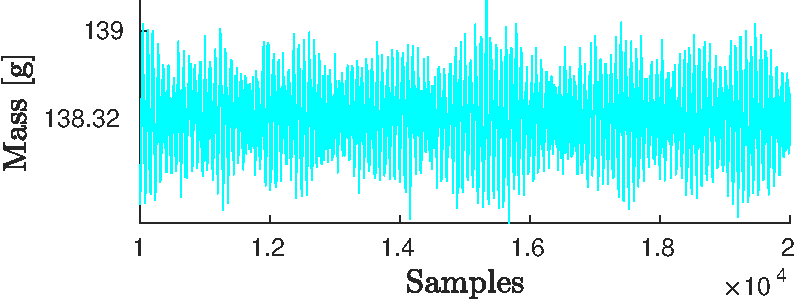
\includegraphics[width=0.6\columnwidth]{../Gus-thesis/ChapterRampInput/fig/Fig_7.pdf} 
    \caption{ \label{fig:rele_lo_40dB_s10} The affine input parameters and the sensor's initial conditions are estimated with the ML method. After three iterations, \color{blue} the average of the relative error is smaller than 5 \% for each and everyone of the estimates. The estimate $\widehat{x}_{\mathrm{ini,2}}$ has the larger relative error near to 1 \%. \color{black} }
    \end{figure}

    Figure \ref{fig:cov_lo_40dB_s1} shows \color{blue} the average \color{black} of the variances that were observed on the diagonal of the covariance matrix $\mathbf{J}$. 
    We can see that the estimation variances decrease as more samples are processed.
    Moreover, the estimation variances of $\widehat{a}$ and $\widehat{b}$ obtained with the ML method are lower than the corresponding estimation MSE errors obtained from a Monte Carlo simulation of the subspace method.

    \renewcommand{\thefigure}{6.9}
    \begin{figure}[!htbp]
    \centering
    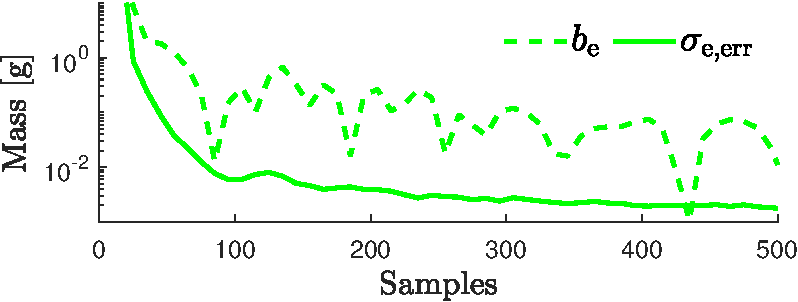
\includegraphics[width=0.6\columnwidth]{../Gus-thesis/ChapterRampInput/fig/Fig_8.pdf} 
    \caption{ \label{fig:cov_lo_40dB_s1} The variances of the ML estimates are calculated using the information provided by the analytic Jacobian. \color{blue} The estimates $\widehat{x}_{\mathrm{ini,1}}$ and $\widehat{a}$ have the smaller and larger variances, respectively. \color{black}  }
    \end{figure}

    \color{black} 

\end{itemize}

\section*{Stephane Chretien}

\begin{itemize}
	\item The Taylor expansion is computed of order 2, what is the accuracy of expansion with respect to system, noise level,... Can you come up with a priori bound on error that will allow you to assess the quality of the expansion? Can you predict where the solution is going to be before computing Taylor expansion?
	
	{\bfseries An a priori bound on the error introduced by the Taylor series expansion can be obtained in terms of the spectral radius of the matrix $\mathbf{M}$. In Section 4.1 the following description has been added: }
	
    \color{blue} An a priori bound on the error introduced by the second order Taylor series expansion can be expressed in terms of the spectral radius $\rho(\mathbf{M})$.
    Considering that the Taylor series expansion is an infinite sum we have that
    \begin{equation} \tag{4.4} \begin{aligned} (\mathbf{I} + \mathbf{M})^{-1} &= \mathbf{I} - \mathbf{M} + \mathbf{M}^2 - \mathbf{M}^3 + \ldots \\
    &=  \mathbf{I} - \mathbf{M} + \mathbf{M}^2 - \mathbf{M}^3 \left( \mathbf{I} - \mathbf{M} + \mathbf{M}^2 - \mathbf{M}^3 + \ldots \right) \\
    &=  \mathbf{I} - \mathbf{M} + \mathbf{M}^2 - \mathbf{M}^3  (\mathbf{I} + \mathbf{M})^{-1} \end{aligned} \end{equation} 
    Therefore we can obtain a bound for the second error expansion error if we take a matrix norm as follows
    \begin{equation} \tag{4.5} \begin{aligned} \| (\mathbf{I} + \mathbf{M})^{-1} - ( \mathbf{I} - \mathbf{M} + \mathbf{M}^2 ) \| &=  \| \mathbf{M}^3  (\mathbf{I} + \mathbf{M})^{-1} \| \\
    & \leq \| \mathbf{M}^3 \| \| (\mathbf{I} + \mathbf{M})^{-1} \| \leq \dfrac{\| \mathbf{M} \|^3}{ 1 -  \| \mathbf{M} \|} = \dfrac{\rho(\mathbf{M})^3}{1 - \rho(\mathbf{M})}  \end{aligned} \end{equation} 
	\color{black}
	
	\item  Concerning other sorts of prior estimations, e.g., given by explicit function theorems. I wonder if you could get something and apply this bound in order to control the bound of the 2nd order expansion. There exist some good results that could help you devise something a priori which can control the error you are making. Neuberger's results (quite old now) but may be handy for this kind of problem. This can be investigated further.
	
	\color{blue}
	Neuberger's paper \cite{Neuberger07} introduces five theorems that are consequence of the continuous Newton method.
	The Newton method aims to find a zero of the function $F: R^n \rightarrow R^n$ by iterating
	\begin{equation} z_{k+1} = z_k - \left(F' (z_k) \right)^{-1} F(z_k) \end{equation}
	for $k=0,1,2,\ldots$, and for a given initial $z_0$, assuming that $\left(F' (y) \right)^{-1}$ exists for some $y \in R^n$.
	A domain of attraction is the set of all initial values $z_0$ that lead to a root of $F$ after the convergence $z_0, z_1, z_2,\ldots$.
	The damped Newton method  
	\begin{equation} z_{k+1} = z_k - \delta_k \left(F' (z_k) \right)^{-1} F(z_k) \end{equation}
	prevents convergence issues, such as chaotic domains of attraction, with $\delta_1, \delta_2, \ldots \in (0, 1)$. 
	The continuous Newton method is a sequence of damped Newton methods. To implement the continuous Newton method, select $T>0$ and perfom $m$ runs of the damped Newton method with $\delta_k = T/m$, for $k=1,2,\ldots, m$.
	The result $z_{k+1}$ is the zero estimation $x_m$, and if the sequence of estimates $x_1, x_2, \ldots$ converges, then it converges to the result of the continuous Newton method.
	
	The objective of the continuous Newton method is to find a function $z: [0, \infty) \rightarrow R^n$, so that
    \begin{equation} z(0) = x \in R^n, \quad z' (t) = - \left(F' (z(t)) \right)^{-1} F(z(t)), \quad t \geq 0, \label{eqn:contNewton}\end{equation}
    subject to the existence of the limit $u=\mathrm{lim}_{t \rightarrow \infty}{z(t)}$, that satisfies $F(u)=0$.
    This implies 
    \begin{equation}  F' (z(t)) z' (t) = - F(z(t)) , \end{equation}
    that is equivalent to
    \begin{equation}  \left(F \circ z\right)' (t) = - F(z(t)) , \end{equation}
    from where we get
    \begin{equation}  F(z(t)) = e^{-t} F(z(0)) . \end{equation}
    Thus, the residual $F(z(t))$ only changes in magnitude and not in direction.
    This property is essential for the results of the theorems in \cite{Neuberger07}. 
    In particular, Theorem 5 gives the conditions for the continuous Newton method to ensure finding a root of the function.
    
    \begin{customthm}{5} \label{thm:five}
    Suppose that each of $H$, $J$, and $K$ is a Banach space, with $H$ compactly embedded in $J$, that $r>0$, and that $G:B_r(0) \rightarrow K$ is continuous as a function on $J$. Suppose also that $g$ belongs to $K$ and that for each $y$ in $b_r(0)$ there is an $h$ in $B_r(0)$, where $b_r(0)$ and $B_r(0)$ are open and closed balls in $H$ of radius $r$ centered at 0, such that
    \begin{equation} \lim\limits_{t \to 0+} -{\dfrac{1}{t} \left(G(y+th) - G(y)\right) = g}. \end{equation}
    Then, there exists $u$ in $B_r(0)$ such that $G(u)=g$.
    \end{customthm}
    %$F:B_r(0) \rightarrow K$
    
    The theorem implies that $u$ is a zero of the function  defined as $F(y) = G(y) - g$.  
    Since $G$ is a continuous function and if $\left(G' (y) \right)^{-1}$ exists for each $y$ in $B_r(0)$, a metric for the validity of the Theorem (\ref{thm:five}) hypothesis is the inequality $\left\Vert  \left( G' (y) \right)^{-1} g \right\Vert \leq r$.
    
    To link the data-driven step-input estimation problem with this theorem, we can take the system of linear equations $\widetilde{\mathbf{y}} = \widetilde{\mathbf{K}} \bm{\theta}$, then define $G(y) = \widetilde{\mathbf{K}} \bm{\theta}$, and $g = \widetilde{\mathbf{y}}$, so that we have $F(\bm{\theta}) = G(\bm{\theta}) - g$. The derivative of the function $G(\bm{\theta})$ is given by $G'(\bm{\theta}) = \widetilde{\mathbf{K}} \mathbf{I}$. Using the pseudo-inverse of $\widetilde{\mathbf{K}}$, the metric $\left\Vert  \widetilde{\mathbf{K}}^{\dagger} \widetilde{\mathbf{y}} \right\Vert \leq r$ indicates that the estimate $\hat{\bm{\theta}}$ is found inside a ball of radius $r$.
    Thus,  
	\color{black}
	
	\item  About trying to find a good transformation from LS to EIV model. I am wondering if you can think of other more accurate starting points instead of LS. Closer to the problem you want to study, but still preserving computational lightness? The closer you start from objective, better the Taylor expansion would be.. Something to investigate as well...
	\item  About robustness: is it an issue in practical problems with heavy tailed noise, outliers,... Perhaps the use of median of means plugged into your approach might produce interesting alternatives for outliers or heavy tailed data. But this is an intricate thing to deal with. Might be interesting to ponder this in future.
	\item  On deep learning: could this be an alternative?
\end{itemize}

\section*{Guillaume Mercere}

\begin{itemize}
	\item In the first or second sentence: “users cannot wait for a steady state regime” . Do you have specific examples of real industrial systems for which it is necessary to have continuous read-out before steady-state is reached? - Further on the industrial part and selling sensors with data-driven parts. Can you explain to experts that your solution is better? Sensors will be used for ages; why not spend one day to do system identification and get a reliable model to make a compensator, instead of using your approach?
	
	{\bfseries The fast weighing of parcels in the post office is a typical example of the real life systems where the time is limited to perform the measurements. Another one that we see nowadays is the temperature measurement of people in airports or train stations to prevent the spread of corona virus. The data driven method can be implemented in portable devices with limited computational resources. In industrial plants were a time slot can be devoted to identify the measurement system and implement a compensation method, the solution might be useful only for a certain amount of time. It is assumed that the model approximation deviates due to changes in the system elements, leading to inaccuracies in the inpiut estimation. There is a need for adaptive methods to avoid stopping the production lines to repeat the system identification procedure. The data-driven method is such an adaptive method. }
	
	\item  Chapter 2, Section 2.2.1. Can you give me some classic solutions/algorithms instead of LS in general? (Say I'm not familiar with EIV or TLS?) Usually with LS problems: multiply with $K^\top$ and compute pseudoinverse. Do you know another solution where they don't use K on the left-hand-side but something else? To get rid of noise by using a matrix on the left-hand-side, is related to EIV. There are some recursive solutions for this. It could be interesting to compare with such IV solutions.
	\item  In Chapter 3: at beginning you say to use linear systems theory to model a sensor. Can you discuss this assumption: is it true in practice? Can you guarantee it behaves like an LTI system?
	\item  Equation 3.1: an LTI system, described with SS representation. You only put output noise on this representation. People sometimes also add process noise. Why? How to modify your approach if there is process noise? Is it still white in this case?
	\item  On page 12 standard approach top of page equation: there are some mistakes in the equations! there is no epsilon (noise) in the equation. But then you do an SVD of H and estimate from there. How does it work if you have noise? Have you tried implementing it and see what you get?
	
	{\bfseries The step input estimation based on singular value decomposition works only with exact data. When  noise perturbes the sensor response the method cannot guarantee the step input estimation. The singular value decomposition of a Hankel matrix constructed from a perturbed sensor response provides only an approximation of the singular values and the singular vectors of this Hankel matrix. Then, the step input estimation obtained with this method from perturbed sensor response is only a rough estimation.     }
	
	\item  On page 12: I’m not sure the equations at the end of the page are correct, e.g., Y=G ubar ... not sure there is x; same for rest; There seem to be many mistakes here and next pages. Be careful with the equations!
	
	{\bfseries The equations have been reviewed and the typos were corrected.}
	
	\item  On page 13, you assume persistency of excitation of order $L$. How do you check this? In your case the input is constant; how to guarantee that the assumption is met?
	
	{\bfseries The persistency of excitation of a signal is verified by looking at the rank of the Hankel matrix constructed from the consecutive samples of this signal. When the Hankel matrix of $L+1$ block rows has a rank lower or equal than L, then we say that the signal is persistently exciting of order $L$. A step input has a very low order of persistency $L=1$, but the step respose of a system has a larger order of persistency. In fact, we assume that if the persistency of excitation of the step response is sufficiently high, then the columns of the Hankel matrix constructed from the step response span a linear space with all the responses of the equivalent augmented autonomous system where the step input is considered an augmented initial condition.}

	\item  In Chapter 4, p 17, Section 4.1.1: You assume that perturbations are IID and must be normally distributed. Why using an assumption of normally distributed? I would think that the kind of distribution is important for CRLB, but I’m not sure you need it for eqns 4.8, 4.9, 4.10,... IID is important, normality perhaps not.
	
	{\bfseries The following paragraph has been added in Section 4.1 to discuss on the need for the normality assumption.  }
	
	\color{blue}
	The normality assumption is necessary to provide more prior information into the method formulation.
    The second order Taylor series expansion (4.4) is developed considering the perturbation noise that gets into the regression matrix from the sensor transient response.
    Assuming only that the perturbation noise is distributed with zero mean and variance $\sigma_{\bm{\epsilon}}^2$ is not enough.
    If we additionally assume normality for the perturbation noise, then we benefit from the knowledge of the third moment equal to zero due to symmetry, and the fourth moment equal to three times the squared variance, which can be disregarded since $3 \sigma_{\bm{\epsilon}}^4 \ll \sigma_{\bm{\epsilon}}^2$\color{black}.
	
	\item   In equation 4.11 you have $\sigma_eps^2 + \sigma_e^2$; how to get in practice $\sigma_e$? Do you have to do this each time? Recursively?
	
	{\bfseries The measurementy noise variance is prior information and in Chapter 5 we describe two ways of estimating $\sigma_{\bm{\epsilon}}$ In summary, the measurement noise can be extracted fom the sensor ressponse once the transient effects are smaller than the noise floor, or from the sensor response power spectrum. The online estimation of the measurement noise, simultaneously with the online step input estimation is a topic for future research.   }
	
	
	\item   Switch to 4.2, simulation results: first part dedicated to K, randomly generated; not sure if still possible, but in all your results it would be nice to have somewhere explicitly K = ... (even if randomly generated). You use only one realization also for matrices A, B, C, D in the text, so it can be added explicitly.
	\item   in Fig 4.1 the bottom figure also discusses the structured case. Why do you talk about structured results in a section about the unstructured case?
	
	{\bfseries Section 4.2 has been improved to describe the result next to its discussion.  }
	
	\item   In 4.1 uses a constant K, but in 4.2.2 you use A, B, C, D, without any links to K. You compare the two curves generated from different data sets… It is strange to compare them. I don't see the link between both.
	
	{\bfseries Section 4.2 has been reestructured and the simulation for the unstructured case were redone to establish a link between the two cases. The exact data is the same in the two cases and the perturbation noise follows the corresponding rules of each case, with the same variance noise levels. In this way the comparison between the two cases makes more sense.  }
	
	\item   To show comparison between structured and unstructured case, use unstructured results for structured case; then use unstructured results for structured case and cover all the possibilities. Now you compare curves related to two different simulations.
	
	{\bfseries \color{red} Interesting question, I want to try it this evening \color{black}}
	
	\item   I was surprised to read in Chapter 5 something very close to what I read in chapter 4. In both cases generated A, B, C. In 5.1 again oscillating 5th order system, similar conclusions, ... What is the added value of 5.1 wrt 4.2.2?
	
	{\bfseries The derivation described in Chapter 4 was conducted with a second order mass-spring-damper weighing system example on mind, and the results observed were submitted in the corresponding paper. Afterwards, when we moved to the practical implementation, we faced the increase of the model order after setting up the weighing experiment. The lowest order we can assume is fifth order. So we decided to repeat the simulations and these new results serve two purposes: a transition from simulation to experimental results, and also to get an insight on the impact of the bias and variance predictions after increasing the model order.    }
	
	\item   On the impact of selected order on results. You were talking about a related bias/variance trade off. So, do you know in the literature some solutions to avoid overfitting? Can you cite something? Can you use something in your case to test for a good order of system?
	\item   Do you know of cross-validation: split data into two parts or several parts; some for estimation, some for validation? Have you tried this? Can this be used here to select good orders? Better results? Influence of system order on bias/variance; if I only use one dataset it is complicated and usually you can increase complexity to mimic a data set, but to avoid overfitting (too high order) use a test/validation data set. with this i should see what is the best value... Have you tried this?
	\item   In Section 6.2.2. Why do you call it a max likelihood approach? To me it is not one. Why do you call it like this? Where is the likelihood? Depending on which likelihood (eg. Gaussian, ...) it leads to LS. Don't' call it ML if you dont give distributions on ... In this case it is better to call it a nonlinear minimization procedure. Not clear why you call it ML.
	
	{\bfseries The method description in Section 6.2.2 has been modified to explain why the method is a maximum likelihood method.  }
	
	\item   Concerning the ML approach in simulations, you say that it takes 30 seconds to complete. What is done exactly in these 30 seconds; how many samples, realizations,... I am a bit surprised you require 30 sec for 2 parameters.
\end{itemize}


\section*{Nikos Deligiannis}

\begin{itemize}
	\item When solving algorithms. Do you opt for closed-form solutions, or do you use optimization based algorithms? How to solve LS problems? Do you solve them using pseudo-inverse or do you do gradient descent?
	\item  Today there is an overwhelming amount of data sensed and communicated; How would you apply your method in a scenario where dimensionality increases significantly? This relates to the questions of previous jury members; what is the implication of using numerical versus closed form solutions?
	\item  What if the $K^\top K$ matrix is not invertible? What if you have fewer samples than unknowns; what can you do? Solutions that assume structure like in compressed sensing, regularization,... can you use them, what would be the impact of that?
	\item  You mention that you improve complexity with your approach, but I missed a complexity analysis. Did you do this? Anything in processing time, flops,...?
	\item  You mentioned deep learning could be applied; could you show how? An issue is that neural nets are trained in high SNR data, but applied in engineering with lower SNR. This clogs performance; any ideas? Is this a limitation?
	\item  You mention that you consider Kalman filters; have you seen approaches where they write Deep Learning in form of Kalman Filter; Could this be applicable?
	\item  Recommendation: if you revise the thesis: maybe change "I propose" to "we propose".
	
	{\bfseries The formulation “I propose” was replaced by “we propose”. }
	
\end{itemize}

\section*{Philippe Dreesen}

\begin{itemize}
	\item Your main assumption is that a sensor outputs a steady state value that is proportional to the to-be-measured quantity. This means that you assume that the sensor is a linear system. What if this assumption is not met, and the sensor has a saturation for high values? Can you still use your methods?
	\item  Sensors are physical devices and deliver a continuous-time output. The models that you use are in discrete-time. Are there any risks that you miss information by not sampling fast enough?
	
	{\bfseries In Chapter 3 has been added a discussion on the step invariance transformation. This defines the conditions of the input for describing exactly the system dynamics in discrete time after sampling the continuous system response. If the input is stepwise continuous, then the zero order hold sampling of the step response leads to an exact discrete time representation of the system. The method under study in this thesis was developed for step input, then we can rely on the discrete time representation. There exist corresponding invariant transformations for piecewise linear inputs and for piecewise polynomial inputs that lead to exact representations from first and second order sampling of the system response, respectively.  }
	
	\item  Related to earlier questions about compressed sensing. There are some recent results on the connections between sparsity and low-rank Hankel matrix completion and approximation. Say that you have an issue with missing data, e.g., from sensor outages. Would it be possible to plug in a procedure that does structured matrix completion and approximation into your methods?
\end{itemize}

\section*{Roger Vounckx}

\begin{itemize}
	\item Two practical questions. On page 35-49 you consider a weight of 138.x grams. You sample relatively slowly (4 kHz) and after 500 samples we can consider that we have correct estimation. If I have a container that fills up and weight is constantly changing. Can we tackle this?
	\item  Consider an optical fiber link with a detector capable of 100 million measurements per second. Can I speed up the link by using your method? You have to do calculations: how high can you go in speed before running into troubles with DSP?
\end{itemize}

\section*{Rik Pintelon}

\begin{itemize}
	\item Returning to a question by Guillaume Mercere: on page 17; do you need normality? You made 2nd order taylor series expansion. Which moment do you need to estimate? Look at the equations page 16. There are 3rd, 4th order moments,... you need to know something more about the noise; this is one of the reasons to make Gaussian assumption: 3rd order moment is 0 (symmetry); 4th order for Gaussian is easy to have an explicit relationship.
	
    {\bfseries Section 4.1 has been appended with a paragraph to discuss on the need for the normality assumption.  }

	\item  Returning to a question by Philippe Dreesen on missing data. If you can deal with missing data, you can deal with saturation in sensors: you just remove the saturations. What is the rank of the Hankel matrix? Is it full rank or not? The question is if matrix completion can help? It works in low-rank approximations; not if the matrix is of full rank.
\end{itemize}

\section*{Ivan Markovsky}

\begin{itemize}
	\item About scalability of algorithms: You said in the very beginning that it can be very fast compared with system identification. This is the point: can you think of a good answer for these questions on scalability? Nikos Deligiannis mentioned computational analysis. You can directly say for (R)LS what is the computational complexity. Order three if full matrix inversion, now per iteration only linear. So you can scale to very large data sizes.
	
	{\bfseries The last paragraphs of Section 3.2 have been included to discuss the scalability of the data-driven step input estimation method.  }

\end{itemize}

\section*{Detailed comments provided by jury members}

\section*{Guillaume Mercere}

\begin{itemize}
	\item It is important for me to know why these new developments are generated. That is the reason why I suggest adding sections or paragraphs dedicated to
    \begin{itemize}
        \item the reasons why, in the industry, we need such a new technique. As I said during the defense, do you have a list of sensors for which waiting for the steady regime for getting the measurement is not possible? Why do you need a fast algorithm? What are the reasons why industry people need fast algorithms? In the end, it seems that, for you, it is more important to have a fast biased result than an unbiased estimate. Why? What do you mean by fast?
        \item  the literature on EIV estimation problems. As shortly mentioned in Chapter 2, there are solutions in the literature (by the way, you never mention the recent book written by Torsten Soderstrom in your document which is strange for me). But you do not describe them (even shortly) and, more importantly, you do not criticize them. Not in general but, at least, explain why you do not use them, what are their advantages and drawbacks and, finally, w.r.t. this list of positive and negative points, why you choose a (R)LS solution. E.g., why not using a recursive instrumental variable solution instead?
        
        {\bfseries A description of IV methods has been added in Section 4.1.4}
        
        \color{blue}
    \subsection*{4.1.4. Instrumental variables formulation of the data-driven step input estimation method}

    The errors-in-variables problem formulation (3.18) of the data-driven step input estimation method can be converted into an instrumental-variables problem.
    A guide to do this conversion is found in \cite{Soderstrom18} and in \cite{Pintelon12Book}. 
    The instrumental variable $\widetilde{\mathbf{Z}}$ has to be selected so that the normal equations (3.19) are expresed instead as
    \begin{equation} \tag{4.22} \widetilde{\mathbf{Z}}^\top \widetilde{\mathbf{K}} \bm{\theta} = \widetilde{\mathbf{Z}}^\top \widetilde{\mathbf{y}} . \label{eqn:neq_siv} \end{equation}
    The selection of the instrumental variable has to be done in such a way that is correlated the regression matrix $\widetilde{\mathbf{K}}$, and uncorrelated with the perturbations $\bm{\epsilon}$.
    Assuming that the block-Hankel matrix $\widetilde{\mathbf{K}}$ is given by
    \begin{equation} \tag{4.23} \widetilde{\mathbf{K}} = \begin{bmatrix} G & \Delta \widetilde{y}(1) & \Delta \widetilde{y}(2) & \cdots & \Delta \widetilde{y}(n) \\ G & \Delta \widetilde{y}(2) & \Delta \widetilde{y}(3) & \cdots & \Delta \widetilde{y}(n+1) \\ \vdots & \vdots & \vdots & & \vdots \\ G & \Delta \widetilde{y}(n+1) & \Delta \widetilde{y}(n+2) & \cdots & \Delta \widetilde{y}(2n) \end{bmatrix} , \label{eqn:matrixK_r} \end{equation}
    then, the instrumental variable $\widetilde{\mathbf{Z}}$ should not contain the elements that construct $\widetilde{\mathbf{K}}$, i.e., the elements of the vector $\left( \widetilde{y}(1), \ldots, \widetilde{y}(2n+1) \right)^\top$.
    A possibility to generalize this idea is expressing the instrumental variable as
    \begin{equation} \tag{4.24} \widetilde{\mathbf{Z}}(t) = \begin{bmatrix} G & \Delta \widetilde{y}(t-4n) & \Delta \widetilde{y}(t-4n+1) & \cdots & \Delta \widetilde{y}(t-3n-1) \\ G & \Delta \widetilde{y}(t-4n+1) & \Delta \widetilde{y}(t-4n+2) & \cdots & \Delta \widetilde{y}(t-3n) \\ \vdots & \vdots & \vdots & & \vdots \\ G & \Delta \widetilde{y}(t-3n) & \Delta \widetilde{y}(t-3n+1) & \cdots & \Delta \widetilde{y}(t-2n-1) \end{bmatrix} , \label{eqn:matrixZ_t} \end{equation}
    for a regression matrix
    \begin{equation} \tag{4.25} \widetilde{\mathbf{K}}(t) = \begin{bmatrix} G & \Delta \widetilde{y}(t-2n+1) & \Delta \widetilde{y}(t-2n+2) & \cdots & \Delta \widetilde{y}(t-n) \\ G & \Delta \widetilde{y}(t-2n+2) & \Delta \widetilde{y}(t-2n+3) & \cdots & \Delta \widetilde{y}(t-n+1) \\ \vdots & \vdots & \vdots & & \vdots \\ G & \Delta \widetilde{y}(t-n+1) & \Delta \widetilde{y}(t-n+2) & \cdots & \Delta \widetilde{y}(t) \end{bmatrix} , \label{eqn:matrixK_t} \end{equation}
    for $t = 4n+1, \ldots, N$.

    The difference with the EIV formulation is that this implementation of the IV method requires to wait more, until $4n+1$ samples of the sensor response are read, instead of $2n+1$ samples. 
    For sensors of small order this twice-the-time waiting does not represent a big change, but as the sensor order increases, the need for waiting can turn the method into impractical since a lot of time should pass before starting to estimate the input. 
    
    There exists a generalized instrumental variables method (GIVE) that was proposed to identify dynamic models from input/output data. 
    GIVE is a bias-eliminating method that uses a generalized instrumental vector constructed from delayed values of the input and output signals \cite{Soderstrom18}.
    Since the aim of this thesis is to analize a method that directly estimates the input from the observed sensor output, without identifying explicitly a dynamic model of the sensor, the GIVE method is out of the scope of this work. 
    A future research can include studying the formulation of a data-driven input estimation method in the spirit of the GIVE method. 
    Nevertheless, a brief description of the GIVE method and its recursive version is given in the following paragraphs.
    
    \subsubsection*{4.1.4.1 Generalized instrumental variables method}
    For an errors-in-variables problem expressed as
    \begin{equation} \tag{4.26} \widetilde{y}(t) = \widetilde{\bm{\phi}}(t) \bm{\theta}   \end{equation}
    where $\widetilde{y}(t)$ is the output perturbed by measurement noise, $\bm{\theta}$ is the vector of to-be-estimated parameters, and $\widetilde{\bm{\phi}}(t)$ is the regressor vector constructed from delayed samples of the measured input $\widetilde{u}(t)$ and output $\widetilde{y}(t)$.
    The least-squares estimate $\widehat{\bm{\theta}}_{\mathrm{LS}}$ is the solution of the normal equation
    \begin{equation} \tag{4.27} \widehat{\mathbf{R}}_{\widetilde{\bm{\phi}}} \widehat{\bm{\theta}}_{\mathrm{LS}} = \widehat{\mathbf{r}}_{\widetilde{\bm{\phi}} \widetilde{y}} , \label{eqn:norm} \end{equation}
    where $\widehat{\mathbf{R}}_{\widetilde{\bm{\phi}}}$ is the covariance matrix of the regressor vector, and $\widehat{\mathbf{r}}_{\widetilde{\bm{\phi}} \widetilde{y}}$ is the cross-covariance matrix of the regressor vector and the output.
    When the number of samples becomes infinitely large, these covariances matrices can be expressed as a sum of the contributions from exact data and measurement noise contributions
    \begin{equation} \tag{4.28} \begin{aligned}  \lim\limits_{N \rightarrow \infty} \widehat{\mathbf{R}}_{\widetilde{\bm{\phi}}} &= \mathbb{E} \{ \widetilde{\bm{\phi}} \widetilde{\bm{\phi}}^\top \} = \mathbf{R}_{\bm{\phi}} + \mathbf{R}_{\bm{\eta}} \\ \lim\limits_{N \rightarrow \infty} \widehat{\mathbf{r}}_{\widetilde{\bm{\phi}} \widetilde{y}} &= \mathbb{E}\{ \widetilde{\bm{\phi}} \widetilde{y}^\top \} = {\mathbf{r}}_{\bm{\phi} y} + {\mathbf{r}}_{\bm{\eta} \bm{\epsilon}} , \end{aligned} \end{equation}
    where we are assuming that $\widetilde{y} =  y +\bm{\epsilon}$, $\widetilde{\bm{\phi}} = \bm{\phi} + \bm{\eta}$, and $\mathbf{r}_{\bm{\phi} y} = \mathbf{R}_{{\bm{\phi}}} \bm{\theta}$.
    The bias of the least-square solution can be expressed as 
    \begin{equation} \tag{4.29} \mathbf{R}_{\widetilde{\bm{\phi}}} \left( \widehat{\bm{\theta}}_{\mathrm{LS}} - \bm{\theta} \right) = \mathbf{r}_{\widetilde{\bm{\phi}} \widetilde{y}} - \mathbf{R}_{\widetilde{\bm{\phi}}} \bm{\theta} = \mathbf{r}_{\widetilde{\bm{\eta}} \bm{\epsilon}} - \mathbf{R}_{\bm{\eta}} \bm{\theta} , \end{equation}

    If we assume that the measurement noise is white for both the input and output, 
    \begin{equation} \tag{4.30} \mathbf{r}_{\widetilde{\bm{\eta}} \bm{\epsilon}} = \mathbb{E}\{ \bm{\eta} \bm{\epsilon}^\top \} = \mathbf{0} \quad \mathrm{and} \quad \mathbf{R}_{\bm{\eta}} = \begin{bmatrix} \sigma_{\bm{\epsilon}}^2 \mathbf{I}_{n_y} & \mathbf{0} \\ \mathbf{0} & \sigma_u^2 \mathbf{I}_{n_u} \end{bmatrix}, \end{equation} 
    where $\sigma_{\bm{\epsilon}}^2$ and $\sigma_u^2$ are the variances of the output and the input, respectively. The normal equation (\ref{eqn:norm}) implies that 
    \begin{equation} \tag{4.31} \left( \mathbf{R}_{\bm{\phi}} + \mathbf{R}_{\bm{\eta}} \right)  \left( \widehat{\bm{\theta}}_{\mathrm{LS}} - \bm{\theta} \right) \neq \mathbf{0}, \end{equation}
    and the estimate $\widehat{\bm{\theta}}_{\mathrm{LS}}$ is not consistent.
    Instead, a bias-compensating least squares estimation can be obtained with  
    \begin{equation} \tag{4.32} \widehat{\bm{\theta}}_{\mathrm{BCLS}} = \left( \mathbf{R}_{\widetilde{\bm{\phi}}} - \mathbf{R}_{\bm{\eta}} \right)^{-1}  \left(  \mathbf{r}_{\widetilde{\bm{\phi}} \widetilde{y}} - \mathbf{r}_{\bm{\eta} \bm{\epsilon}} \right) . \end{equation}

    To formulate the generalized instrumental variable estimator, a generalized instrumental vector $\mathbf{z}(t)$ is built from delayed samples of the input and the output. 
    The dimension of the generalized instrumental vector should be $n_{\mathbf{z}} \geq \mathrm{dim} ( \vartheta ) = n_u + n_y + 2$, since the total parameter vector $\vartheta = \left( \theta^\top, \rho^\top \right)^\top$ considers also the variances of the measurement noise $\rho = \left( \sigma_{\bm{\epsilon}}^2, \sigma_u^2 \right)^\top$. 
    Since the generalized instrumental vector $\mathbf{z}(t)$ and the equation error $\widetilde{y}(t) - \widetilde{\bm{\phi}}(t) \bm{\theta}$ must be correlated, we can express the sistem of equation as 
    \begin{equation} \tag{4.33}\left( \mathbf{R}_{\widetilde{\mathbf{z}} \widetilde{\bm{\phi}}} - \mathbf{R}_{\bm{\zeta} \bm{\eta}} \left( \bm{\rho} \right) \right) \bm{\theta} = \left(  \mathbf{r}_{\widetilde{\mathbf{z}} \widetilde{y}} - \mathbf{r}_{\bm{\zeta} \bm{\epsilon}} \left( \bm{\rho} \right) \right) , \label{eqn:GIVE} \end{equation}
    where $\widetilde{\mathbf{z}} = \mathbf{z} + \bm{\zeta}$.

    \subsubsection*{4.1.4.2 Recursive generalized instrumental variables method}
    If we define
    \begin{equation} \tag{4.34} \begin{aligned} \mathbf{h} \left( \bm{\rho}, \bm{\theta} \right)  &=  \mathbf{r}_{ \bm{\zeta} \bm{\epsilon}} \left( \bm{\rho} \right) - \mathbf{R}_{\bm{\zeta} \bm{\eta}} \left( \bm{\rho} \right) \bm{\theta}  =  \mathbf{J} \left( \bm{\theta} \right) \bm{\rho}, \\
    \mathbf{R} \left( t \right)  &=  \dfrac{1}{t} \sum_{\tau-1}^{t} \widetilde{\mathbf{z}} \left( \tau \right) \widetilde{\bm{\phi}}^\top \left( \tau \right) , \\     
    \mathbf{q} \left( t \right)  &=  \dfrac{1}{t} \sum_{\tau-1}^{t} \widetilde{\mathbf{z}} \left( \tau \right) \widetilde{y} \left( \tau \right) \\     
    \mathbf{b} \left( t \right)  &=  \mathbf{q} \left( t \right) - \mathbf{h} \left( \bm{\rho}, \ \bm{\theta} \right)
    , \end{aligned} \end{equation}
    then the equation (\ref{eqn:GIVE}) is equivalent to
    \begin{equation} \tag{4.35} \mathbf{R} \left( t \right) \bm{\theta} = \mathbf{b} \left( t \right) . \end{equation}
    This representation allows a recursive form
    \begin{equation} \tag{4.36} \begin{aligned} 
    \mathbf{R} \left( t+1 \right)  &= \mathbf{R} \left( t \right) + \dfrac{1}{t+1} \left( \widetilde{\mathbf{z}} \left( t+1 \right) \widetilde{\bm{\phi}}^\top \left( t+1 \right) - \mathbf{R} \left( t \right) \right), \\
    \mathbf{b} \left( t+1 \right)  &= \mathbf{b} \left( t \right) + \dfrac{1}{t+1} \left( \widetilde{\mathbf{z}} \left( t+1 \right) \widetilde{y} \left( t+1 \right) - \mathbf{b} \left( t \right) - \mathbf{h} \left( \bm{\rho}, \ \bm{\theta} \right) \right), \\
    \widehat{\bm{\theta}} \left( t+1 \right)  &=  \left( \mathbf{R}^\top \left( t+1 \right) \mathbf{R} \left( t+1 \right) \right)^{-1} \mathbf{R}^\top \left( t+1 \right) \mathbf{b} \left( t+1 \right) \\
    \mathbf{q} \left( t+1 \right)  &= \mathbf{q} \left( t \right) + \dfrac{1}{t+1} \left( \widetilde{\mathbf{z}} \left( t+1 \right) \widetilde{y} \left( t+1 \right) - \mathbf{q} \left( t \right) \right) \\
    \widehat{\bm{\rho}} \left( t+1 \right)  &=  \mathbf{J}^\dagger \left( \widehat{\bm{\theta}} \left( t \right) \right) \left( \mathbf{q} \left( t \right) - \mathbf{R} \left( t \right) \widehat{\bm{\theta}} \left( t \right) \right) , \end{aligned} \end{equation}
    where $\mathbf{J}^\dagger \left( \widehat{\bm{\theta}} \left( t \right) \right)$ is the pseudo-inverse of $\mathbf{J} \left( \bm{\theta} \right)$.

    The complexity of this recursive generalized instrumental variables estimator is ${O}(n^3)$, that is larger than the ${O}(n^2)$ of the recursive least squares.
    Another drawback of the recursive generalized IV estimator is that it computes a pseudo-inverse matrix in each iteration step.
    If we would need to formulate the data-driven step input estimation problem in the generalized IV framework, it would require to study the formulation in detail because currently the IV framework is based on the assumption that both measurements of the input and output are available, but for the step input estimation problem only the output is available.
    Therefore, it is not straightforward to implement the recursive generalized IV estimator to estimate the step input, and this can lead to future research.
    \color{black}

    \end{itemize}
    \item In the document, you always talk about recursive implementations of least squares solution but, in the end, you never give access to any recursive algorithm description (as you do for what you call the ML method). Why? Do it as well for the recursive weighted least squares solution. 
    
    {\bfseries The following recursive least-squares algorithm description has been added to Section 3.2:}
    
    \color{blue} 
    The problem (3.17) admits a least-squares (LS) solution with normal equations given by
    \begin{equation} \tag{3.19} \widetilde{\mathbf{K}}^\top \widetilde{\mathbf{K}} \bm{\theta} = \widetilde{\mathbf{K}}^\top \widetilde{\mathbf{y}}.   \end{equation} % \label{eqn:neq_seiv} 
    The closed form of the LS solution can be expressed as
    \begin{equation} \tag{3.20} \widehat{\bm{\theta}} = \widetilde{\mathbf{K}}^\dagger \widetilde{\mathbf{y}} = ( \widetilde{\mathbf{K}}^\top \widetilde{\mathbf{K}} )^{-1} \widetilde{\mathbf{K}}^\top \widetilde{\mathbf{y}} , \label{eqn:xhat} \end{equation}
    where $\widetilde{\mathbf{K}}^\dagger$ is the pseudo-inverse matrix of $\widetilde{\mathbf{K}}$.
    As the number of samples $N$ increases, the number of rows of the matrix $\widetilde{\mathbf{K}}$ grows, making the pseudo-inverse computation inefficient since it requires larger flops, memory and time.

    For metrology applications, it is desired to have a fast solution that can be obtained in real-time. 
    The recursive algorithm (RLS) is a least-squares alternative to implement the step input estimation method in real-time.
    The RLS recursively updates the solution of the system of equations, for each newly acquired sensor response sample, considering the previous value of the estimation, instead of performing a matrix inversion.
    An expression of the RLS equations is given in \cite{Kailath00book} as
    \begin{equation} \tag{3.21} \begin{aligned} \widehat{\bm{\theta}}(t) &= \widehat{\bm{\theta}}(t-1) + \bm{\kappa}_{t} \left( \widetilde{y}(t) - \widetilde{k}_{t} \widehat{\bm{\theta}}(t-1) \right) , \\  \bm{\kappa}_{t} &= \bm{\Psi}(t-1) \widetilde{k}_{t}^\top / \left( 1 + \widetilde{k}_{t} \bm{\Psi}(t-1) \widetilde{k}_{t}^\top  \right) \\ \bm{\Psi}(t) &= \left( \mathbf{I} - \bm{\kappa}_{t} \widetilde{k}_{t} \right) \bm{\Psi}(t-1), \label{eqn:RLS} \end{aligned} \end{equation}
    where $\widetilde{k}_{t}$ represents the row of $\widetilde{K}$ that corresponds to the $t\mathrm{-th}$ sample, $\bm{\kappa}_{t}$ is a gain scalar, $\Psi(t)$ is a covariance matrix, and the estimates and the covariance matrix are initialized respectively with $\widehat{\bm{\theta}}(1)= \widehat{\bm{\theta}}(0)$ and $\Psi(-1) = \Psi(0)$.
    Since the RLS is a recursive implementation of the least-squares computation, the RLS solution is equivalent to the LS solution.
    Moreover, the statistical analysis of the LS solution is valid also for the RLS solution, and is preferred since it is simpler to express the statistics using the closed form of the LS solution.    
    \color{black}	
    
    {\bfseries The following description for the exponentially recursive least-squares algorithm has been added to Section 6.2.1:}    

    
    \color{blue}
    The exponentially weighted recursive least-squares (RLS) can solve recursively the estimation problem (3.20).
    In \cite{Kailath00book} is described the exponentially weighted RLS algorithm, which is as follows

    \begin{equation} \tag{6.4} \begin{aligned}  \widehat{\bm{\theta}}(k) &= \widehat{\bm{\theta}}(k-1) + \bm{\kappa}_{k} \left( \widetilde{y}(k) - \widetilde{\mathbf{k}}_{k} \widehat{\bm{\theta}}(k-1) \right) , \\  \bm{\kappa}_{k} &= \omega^{-1} \bm{\Psi}(k-1) \widetilde{\mathbf{k}}_{k}^\top / \left( 1 + \omega^{-1} \widetilde{\mathbf{k}}_{k} \bm{\Psi}(k-1) \widetilde{\mathbf{k}}_{k}^\top  \right) \\ \bm{\Psi}(k) &= \omega^{-1} \left( \mathbf{I} - \bm{\kappa}_{k} \widetilde{\mathbf{k}}_{k} \right) \bm{\Psi}(k-1), \label{eqn:RLS} \end{aligned} \end{equation}
    for $k = 2n+1, 2n+2, \ldots$, where $\widetilde{\mathbf{k}}_{k}$ represents the row of $\widetilde{\mathbf{K}}$ that corresponds to the $k\mathrm{-th}$ sample, $\bm{\kappa}_{k}$ is a gain scalar, and $\Psi(k)$ is a covariance matrix.
    The estimates and the covariance matrix are initialized using the first $n+1$ samples, i.e.,  
    \begin{equation} \tag{6.5} \begin{aligned} \widehat{\bm{\theta}} (2n+1) &= \left( \widetilde{\mathbf{K}}_{n+1}^\top  \bm{\Omega} \widetilde{\mathbf{K}}_{n+1} \right)^{-1} \widetilde{\mathbf{K}}_{n+1}^\top \bm{\Omega}  \widetilde{\mathbf{y}}_{n+1}, \quad \mathrm{and} \\ \Psi(2n+1) &= \left( \widetilde{\mathbf{K}}_{n+1}^\top \bm{\Omega} \widetilde{\mathbf{K}}_{n+1} \right)^{-1} , \end{aligned} \end{equation} 
    where $\widetilde{\mathbf{K}}_{n+1}$ is the matrix $\widetilde{\mathbf{K}}$ with the first $n+1$ rows, and $\widetilde{\mathbf{y}}_{n+1}$ is the vector $\widetilde{\mathbf{y}}$ with the first $n+1$ elements.
    When $\omega=1$, the exponentially weighted RLS solution is identical to that of the RLS.
    When $\omega<1$, the older residuals are weighted with lower values than the residuals of recent observations.
    In this way, the solution of the minimization problem depends more on newer data, and less on older data. 

    \color{black}


    \item Double check your equations page 12 and 13. By the way, can you explain where Eq. (3.6) comes from?
    
    {\bfseries The equations in page 12 and 13 have been reviewed and typos corrected. The derivation of Eq. (3.6) has been improved with more explaination: }
    
    \color{blue}
    A third method can directly estimate the input step level from the step response, without identifying a sensor model.
    To derive this method, we use the first difference operator, $\Delta = \sigma - 1$, where $\sigma$ is the shift operator, defined as $(\sigma^\tau y) (k) = y(k + \tau)$.
    Applying the first difference operator to the system state-space representation (3.1) results in the autonomous system
    \begin{equation} \tag{3.10} \begin{aligned} \Delta \mathbf{x}(k+1) = \mathbf{A} \Delta \mathbf{x}(k), \quad \Delta {y}(k) = \mathbf{C} \Delta \mathbf{x}(k), \quad \text{with} \quad \Delta \mathbf{x}_{\text{ini}} = \Delta \mathbf{x}(0) , \label{eqn:ssalti} \end{aligned} \end{equation}
    where $\Delta {u}(k) = \mathbf{0}$, for $k \geq 0$, and
    $\Delta \mathbf{x}(0) = (\mathbf{A} - \mathbf{I}) \mathbf{x}(0) + \mathbf{B} {{u}}$.

    If the response $\Delta {y}$  of this autonomous system is persistently exciting of order $L$, then the rank of the Hankel matrix $\mathbfcal{H}_{L+1}(\Delta {y})$ of $L+1$ block rows constructed from $\Delta {y}$ satisfies
    \begin{equation} \tag{3.11} \mathrm{rank} \left( \mathbfcal{H}_{L+1} \left( \Delta {y} \right) \right) = \mathrm{rank} \left( \begin{bmatrix} \Delta y(1) & \Delta y(2) & \cdots & \Delta y(n) \\ \Delta y(2) & \Delta y(3) & \cdots & \Delta y(n+1) \\ \iddots & \iddots & \iddots \\ \Delta y(L+1) & \Delta y(L+2) & \cdots & \Delta y(L+n) \end{bmatrix} \right) \leq L,  \end{equation}
    and the Hankel matrix $\mathbfcal{H}_{L+1}(\Delta {y})$ is a linear map to the natural responses of the augmented autonomous system (3.3) 
    \begin{equation} \tag{3.12} \mathbf{y}_{\mathrm{natural}} = \mathbfcal{H}\left(\Delta {y}\right) \bm{\ell}, \end{equation}
    from any vector $\bm{\ell} \in \mathbb{R}^{n}$.
    The total response of the system is the sum of the forced response, due to the applied input ${u}$ and the natural response
    \begin{equation} \tag{3.13} \mathbf{y} = \mathbf{y}_{\mathrm{forced}}+ \mathbf{y}_{\mathrm{natural}} =G {u} + \mathbfcal{H}\left(\Delta {y}\right) \bm{\ell} ,  \end{equation} 
    that is equivalent to
    \begin{equation} \tag{3.14} \underbrace{ \begin{bmatrix} y(n+1) \\ \vdots \\ y(N) \end{bmatrix}}_{\mathbf{y}} = \underbrace{ \begin{bmatrix} G & \Delta y(1) & \Delta y(2) & \cdots & \Delta y(n) \\ G & \Delta y(2) & \Delta y(3) & \cdots & \Delta y(n+1) \\ \vdots & \iddots & \iddots & \iddots \\ G & \Delta y(N-n) & \Delta y(N-n+1) & \cdots & \Delta y(N-1) \end{bmatrix} }_{\mathbf{K}} \underbrace{ \begin{bmatrix} {{u}} \\ \bm{\ell} \end{bmatrix} }_{\bm{\theta}} , \label{eqn:ddsiemexd} \end{equation}
    where $N$ is the number of samples.
    From this point of view, the vector $\bm{\ell}$ is a linear transformation of the system's initial conditions.  
    \color{black}
    
    \item  In Section 4.1.1 and 4.1.2, discuss the normality assumption. Please restructure Section 4.1.3 which is not clear for me. 
    
    {\bfseries The discussion of the normality assumption has been added to Section 4.1, since it is relevant for the two cases considered. Section 4.1.3 has been reestructured to improve its clarity.}
    
    \item  Why do you always study the statistical properties of your least squares solution with high SNR only? What do you get for SNR = 10 dB for instance? 
    \item Give the values of the matrices you use for simulating data sets so that the reader can test what you have carried out. 
    
    {\bfseries The first paragraphs of Section 4.2, and Fig. 4.1, were added to describe the conditions in which the simulations were conducted from the structured and unstructured EIV problems.}

    \color{blue}
    Two Monte Carlo (MC) simulation studies were conducted to test the obtained bias and variance formulas.
    There are two sets of formulas.
    One set was obtained for the unstructured and uncorrelated EIV problem, and, the other set, for the structured and correlated EIV problem. 
    The problem solved by the data-driven step input estimation method (3.20) belongs to the second set.
    The objective of the MC simulations is to compare the results of the bias and variance formulas in these two cases. 
    The comparison is an evaluation of the effect that the structure and correlation have in the problem solution.
    To make a fair comparison, the same exact data and the perturbation variance is used in both types of EIV problems. 

    The exact data is the system of linear equations \ref{eqn:ddsiemexd} built by the data-driven step input estimation method.
    To build the system of equations, the processed signal ${y}$ is the exact response of a sensor to the input $0.1s$, where $s$ is the unit step response.  
    The sensor is modeled as a linear time-invariant mass-spring-damper system of order $n = 2$, that is given by 
    \begin{equation} \tag{4.37}
    \mathbf{x}(k+1) = \begin{bmatrix} 0 & 1 \\ \dfrac{-k_{\mathrm{s}}}{m+M} & \dfrac{-k_{\mathrm{d}}}{m+M} \end{bmatrix} \mathbf{x}(k) + \begin{bmatrix} 0\\ -g\end{bmatrix} u(k),  
    \quad y(k) = \begin{bmatrix} -1 & 0 \end{bmatrix} \mathbf{x}(k), \label{eqn:msdst}
    \end{equation}
    where $m=0.015$ kg, $k_{\mathrm{s}}=500$ kg/m, $k_{\mathrm{d}}=0.5$ kg s/m, $M=0.1$ kg, and $g=9.81 \ \mathrm{m/s^2}$.   
    The exact sensor response is shown in Figure 4.1.

    In the simulations, the sample size considered is $N=200$, since there the transient regime of the sensor model is still evident. 
    In the case of the structured EIV problem, this sample size satisfies the requirements of the data-driven step input estimation method. 
    \color{black}

    
    \item Please remove Fig. 4.1 b from Section 4.2.1 because the top and bottom curves are obtained with different systems and simulation condition. Or explain why you can compare both. It could be interesting to test each time (i.e., in Section 4.2.1 and 4.2.2) the bias and covariance formulas obtained by considering the structured and unstructured EIV problems. 
    
    {\bfseries Fig. 4.1 b has been relocated in its corresponding section. Now it is Fig. 4.7.}
    
    \item  When you generate different simulation examples, explain why the new ones are interesting or, more importantly, what they bring w.r.t. the former simulations results. This is the case for instance when I compare Section 4.2.2 and Section 5.1. 
    \item Except if you can convince me, do not use the name "maximum likelihood" when you do not introduce a likelihood you want to maximize. In Chapter 6, you introduce a nonlinear least squares algorithm, nothing else (see the attached document, Numerical Optimization, Chapter 10).
    
    {\bfseries The method description in Section 6.2.2 has been modified to explain why the method is a maximum likelihood method. The modified paragraphs are as follows: }
    
    \color{blue} 
    Using a model of the sensor, the maximum-likelihood ML method simultaneously estimates the parameters of the applied affine input $u(t) = at + b$, and some of the sensor model parameters, using the observed sensor response $\widetilde{\mathbf{y}}$.
    This method fits iteratively the response of the model $\widehat{\mathbf{y}}(\bm{\theta})$ to the sensor response by searching for the parameters $\bm{\theta}$ that reduce the error difference between both responses.
    Algorithm 6.1 describes the formulation of an objective function $f = \mathbf{r}^\top \mathbf{r}$, where $\mathbf{r}$ is the residual $\mathbf{r}(\bm{\theta}) = \widetilde{\mathbf{y}} - \widehat{\mathbf{y}}(\bm{\theta})$, that is minimized through the iterations.
    The objective function is the sum of the squares of the differences between the samples of both responses.
    Since the measurement noise is assumed Gaussian distributed with zero mean and variance $\sigma_{\bm{\epsilon}}^2$, where the samples of this perturbation are independent and identically distributed, the minimization of the objective function $f$ maximizes the likelihood of fitting the actual sensor response with the model response.


    The Jacobian matrix of the residual $\mathbf{J}\bm{\theta} = \partial \mathbf{r}(\bm{\theta}) / \partial \bm{\theta}$ can be analytically derived using the sensor model.
    With the Jacobian matrix, the ML method searches the direction in which the residual decreases towards a local minimum.
    Unfortunately, this ML method cannot guarantee the global minimum since it depends strongly on the initialization of the optimization parameters, as it is discussed in \cite{Nocedal06}.
    Therefore, it is proposed to initialize the to-be-optimized parameters $a$ and $b$ using the results of the subspace method obtained after a convenient number of samples so that the affine input parameters are set close to the optimal values.
    The initialization of the remaining model parameters under study can be done using the sensor model representation.
    An illustrative example of the ML will be provided in a posterior subsection.  
    \color{black}
\end{itemize}

\section*{Nikos Deligiannis}

\begin{itemize}
    \item Comments related to the structure of the thesis:
    \begin{itemize}
	\item In the introduction chapter it is best to describe a set of applications and settings that motivate your research and proposed solutions. This can make your thesis more accessible. Furthermore, you can add a subsection that describes in a high-level manner the remainder and structure of the thesis (describing briefly the contributions of each chapter). You can also mention your contributions there but in a less technical way since the problem statement only comes in the Chapter preliminaries.
	\item In each main chapter (Chapter 4, Chapter 5, Chapter 6) you can add an introduction subsection, a state-of-the-art subsection and then elaborate your contributions and methods.
    
    {\bfseries The introduction of the chapters now includes the state of the art to position the PhD work with respect to the literature.}

	\item I believe that this structure will improve the understanding of the thesis and light up your contributions.
	
	{\bfseries Indeed, this structure allows to visualize the thesis contributions.}

	\end{itemize}
	\item Further comments:
	\begin{itemize}
	\item Please discuss the complexity and scalability issues related to your approach in relation to the state of the art.
	
    {\bfseries The following paragraph has been added in Section 3.2 to discuss the scalability of the data-driven step input estimation method.}
	
	\color{blue}
    The computational complexity of the RLS algorithm solution to the system of equations (3.14) is $O \left( \left( n+1 \right)^2 \right)$.
    The largest computational requirement is for the initialization of the algorithm, where a matrix inverse is required when the number of samples is just enough to have a square matrix $\widetilde{\mathbf{K}}_{n+1}$.
    From there on, the RLS algorithm updates the solution with linear complexity.
    Therefore, even though a large number of samples $N$ makes the matrix in the system of equations (3.14) increase in the number of rows, the estimation of the solution does not increase in complexity. 
    The data-driven step input estimation method is then scalable for any sensor of order $n$, and can be executed in devices with limited computational resources, provided that the computation of the  $n+1 \times n+1$ inverse matrix is feasible.
    \color{black}
	
	\item Position your work with regard to the state of the art as well as regarding solutions based on low-rank matrix completion and compressed sensing.
	\item I recommend to use the formulation “we propose” than “I propose”
	
	{\bfseries The formulations similar to “I propose” were replaced by equivalents such as “we propose”. }
	
	\item You might wish to add a list of notation in the beginning of the thesis.
	
	{\bfseries A nomenclature list is provided before the summary of the document. }
	
	\end{itemize}
\end{itemize}

\section*{Philippe Dreesen}

\begin{itemize}
    \item General remarks:
    \begin{itemize}
    \item  It would be good to include some layman’s examples that motivate the work of the thesis already in the introduction. In the current text, there is a nice example on page 52, almost at the end of the thesis. These kinds of examples should appear in the introduction to motivate and position the work.
    
    {\bfseries The following paragraphs have been added to the Introduction: }
    
    \color{blue}

    Take for example the case of a thermometer.
    To measure temperature, the thermometer is put in contact with the substance or object of interest.
    Accordingly to the Newton's law of cooling, the temperature $y$ of the thermometer changes proportionally to the its difference with respect to the temperature $u$ of the matter under study:
    \begin{equation} \tag{2.1}  \dfrac{dy}{dt} = k_T \left( u - y \right) \label{eqn:NewtonCooling} \end{equation}
    where the proportionality constant $k_T$ is a parameter of the thermometer first order model.
    The input $u$ is unknown and its estimation is the objective of the measurement.
    It is customary to take the reading from the thermometer once the temperature stops changing. 

    Another popular example of a measurement is found in weighing. 
    In most of modern scales, the object of interest if placed on top of a weighing sensor.
    A simple model of the weighing sensor is the second order mass-spring-damper model shown in Figure \ref{fig:simple_msd_system}.
    In this model, the unknown mass $u$ causes a displacement $y$ of the scale and the dynamics of the sensor are described by the differential equation:
    \begin{equation} \tag{2.2} \dfrac{d}{dt} \left( u(t) \ \dfrac{dy}{dt} \right) + k_{\mathrm{d}} \dfrac{dy}{dt} + k_{\mathrm{s}} y = u(t) \ g \end{equation}
    where $m$ is the own mass of the scale, $k_{\mathrm{d}}$ is the damping constant, $k_{\mathrm{s}}$ is the elasticity constant, and $g = 9.81$ $\mathrm{m/s}^2$ is the gravitational acceleration. 

    For illustration purposes, Figures \ref{fig:thermometer} and \ref{fig:scale} show the responses of the thermometer and the weighing sensors, respectively, after the application of a constant input $u$, which can be represented by a step input. 

    \renewcommand{\thefigure}{2.1}
    \begin{figure}[htb!]
    \centering

    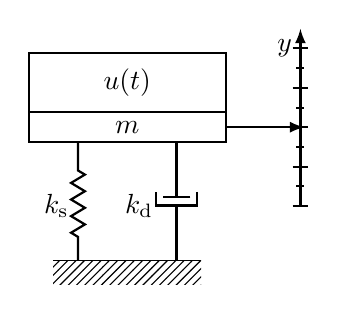
\begin{tikzpicture}[every node/.style={draw,outer sep=0pt,thick}]
    \tikzstyle{spring}=[thick,decorate,decoration={zigzag,pre length=0.3cm,post length=0.3cm,segment length=6}]
    \tikzstyle{damper}=[thick,decoration={markings,  
    mark connection node=dmp,
    mark=at position 0.5 with 
    {
    \node (dmp) [thick,inner sep=0pt,transform shape,rotate=-90,minimum width=15pt,minimum height=3pt,draw=none] {};
    \draw [thick] ($(dmp.north east)+(2pt,0)$) -- (dmp.south east) -- (dmp.south west) -- ($(dmp.north west)+(2pt,0)$);
    \draw [thick] ($(dmp.north)+(0,-5pt)$) -- ($(dmp.north)+(0,5pt)$);
    }
    }, decorate]
    \tikzstyle{ground}=[fill,pattern=north east lines,draw=none,minimum width=0.63cm,minimum height=0.3cm]

    \node (M) [minimum width=2.5cm,minimum height=0.05cm] {$m$};
    \node (Mu) [minimum width=2.5cm,minimum height=0.75cm,yshift=0.57cm] {$u(t)$};

    \node (ground1) at (M.south) [ground,yshift=-1.5cm,xshift=-0.625cm,anchor=north] {};
    \draw (ground1.north west) -- (ground1.north east);
    \draw [spring] (ground1.north) -- ($(M.south east)!(ground1.north)!(M.south west)$);

    \node (groundc) at (M.south) [ground,yshift=-1.5cm,anchor=north] {}; 
    \draw (groundc.north west) -- (groundc.north east);

    \node (ground2) at (M.south) [ground,yshift=-1.5cm,xshift=0.625cm,anchor=north] {};
    \draw (ground2.north west) -- (ground2.north east);
    \draw [damper] (ground2.north) -- ($(M.south east)!(ground2.north)!(M.south west)$);

    \node[draw=none,fill=none] at (-0.9cm,-1cm) {$k_{\mathrm{s}}$};
    \node[draw=none,fill=none] at (0.15cm,-1cm) {$k_{\mathrm{d}}$};
    \node[draw=none,fill=none] at (2.0cm,1.0cm) {$y$};
    \draw [-latex,thick]  ++(2.2cm,-1cm) -- +(0cm,2.25cm);

    \draw [-latex,thick] (M.east) ++(0,0) -- +(1cm,0);
    \draw [line width=0.25mm] (2.2cm,-1cm) -- (2.2cm,1cm);
    \draw [line width=0.25mm] (2.1cm,-1cm) -- (2.3cm,-1cm);
    \draw [line width=0.25mm] (2.1cm,1cm) -- (2.3cm,1cm);
    \draw [line width=0.25mm] (2.1cm,-0.5cm) -- (2.3cm,-0.5cm);
    \draw [line width=0.25mm] (2.1cm,0.5cm) -- (2.3cm,0.5cm);
    \draw [line width=0.25mm] (2.15cm,-0.25cm) -- (2.25cm,-0.25cm);
    \draw [line width=0.25mm] (2.15cm,0.25cm) -- (2.25cm,0.25cm);
    \draw [line width=0.25mm] (2.15cm,-0.75cm) -- (2.25cm,-0.75cm);
    \draw [line width=0.25mm] (2.15cm,0.75cm) -- (2.25cm,0.75cm);
    \draw [line width=0.25mm] (2.1cm,0cm) -- (2.3cm,0cm);

    \end{tikzpicture}

    \caption{\label{fig:simple_msd_system}  \color{blue} A second order mass-spring-damper model represents the weighing sensor. The application of the mass $u$ causes a change in the position $y$ of the scale. \color{black} } 
    \end{figure}


    \renewcommand{\thefigure}{2.2}
    \begin{figure}[!htbp]
    \centering
    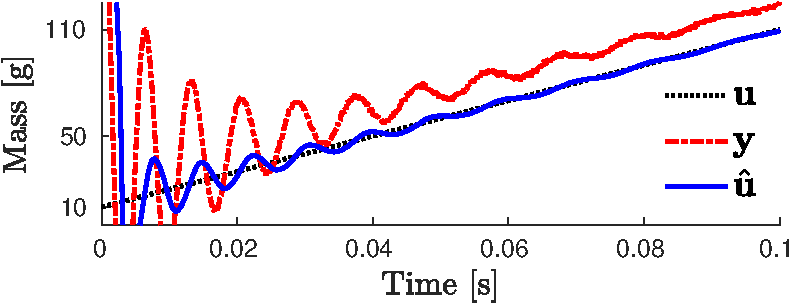
\includegraphics[width=0.6\columnwidth]{../Gus-thesis/ChapterIntroduction/fig/Fig_2.pdf} 
    \caption{ \label{fig:thermometer} 
    \color{blue} This simulation shows an example of the temperature change experimented by a thermometer, with $k_T=0.5 s^{-1}$, caused by applying a step input of 67 $\circ \mathrm{C}$  when the thermometer was initially at 23 $\circ \mathrm{C}$. In this example, we should wait 10 s to have an accurate estimation of the input. \color{black} }
    \end{figure}

    \renewcommand{\thefigure}{2.3}
    \begin{figure}[!htbp]
    \centering
    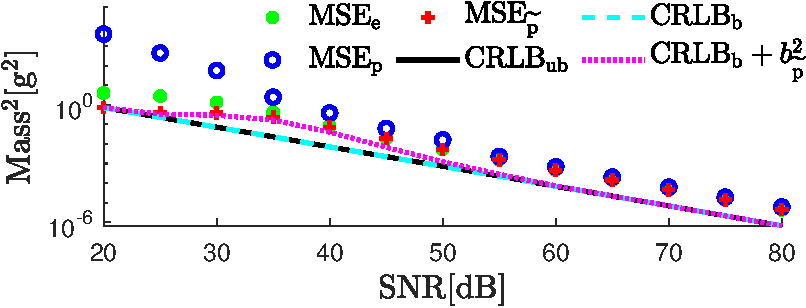
\includegraphics[width=0.6\columnwidth]{../Gus-thesis/ChapterIntroduction/fig/Fig_3.pdf} 
    \caption{ \label{fig:scale} 
    \color{blue} This simulation illustrate the displacement observed when a constant input $u=1 \mathrm{kg}$ is applied to a weighing sensor in equilibrium. The sensor parameters are $k_{\mathrm{d}} = 5 \mathrm{N s/m}$, and $k_{\mathrm{s}} = 10000 \mathrm{N/m}$. In this conditions, the user has to wait more that 2 s to observe a stabilization on the scale and to estimate the mass from reading the final value of the displacement. \color{black}  }
    \end{figure}

    \color{black}

    
    \end{itemize}
    \item Detailed remarks:
    
    {\bfseries The detailed remarks in this list have been attended accordingly: }
    
    \begin{itemize}
    \item Citations that are used in-line should have brackets only around the year, not around the authors’ names. For instance on page 3, line -2 is written “reviewed in [Hack and ten Caten, 2012]”. This should be displayed as “reviewed in Hack and ten Caten [2012]. In LaTeX this can typically be done by making the proper distinction between the commands \ citet and \ citep. The former is used for references in text, the latter for parenthetical references.
    \item  On page 1 of the PDF (front of thesis), I believe also N. Deligiannis should be mentioned with the title “prof.”. 
    \item Page 1 of thesis: typo on line 6: “and on the sensor initial conditions” => “sensor’s initial conditions”
    \item Page 3, line -2: “uncertainty analysis are reviewed” => “is reviewed”
    \item Page 3, line -1: remove comma before “that”
    \item Page 3, line -2: fix the in-text reference (see above)
    \item Page 4, lines 11-13: fix the in-text references (see above)
    \item Page 5, line 5: Remove “The” at the beginning of the sentence (The Hankel…)
    \item Page 6, line 10: fix the in-text references (see above)
    \item Page 7, lines 10-11: the sentence on heart and breathing physiological monitoring sounds a bit awkward. Please reformulate.
    \item Page 9, line -1: fix the in-line reference (see above)
    \item Page 10, lines 1-3: in the enumeration of the types of sensors, remove the article ‘the’ before the sensor name. So: “like three-axis sensors [ref], radio-frequency intruder sensors [ref], and radar sensors [ref]. 
    \item Page 10, equation 3.10: The symbol D was not bold in the equations above. Be consistent!
    \item Page 10, caption of figure: replace “reverts” by “inverts”
    \item Page 11, line 9, put “poles” between parentheses instead of between commas.
    \item Page 12, line -6: “that in matrix form is” => “which in matrix form is”
    \item Page 13, line -9: “in the practice” => “in practice”
    \item Page 14, line -14: missing space between “problem” and “(3.11)”
    \item Page 16, halfway page: the sentence “Applying a second-order…” is not a proper sentence (perhaps fix this by removing “that”).
    \item Page 16 introduces seemingly some new notation, e.g., b(.), mu(.) and C(.). While their meaning is clear from the context, it is desirable to give proper definitions when introducing new mathematical tools.
    \item Page 17, line -1: fix in-text references (see above)
    \item Page 20 (and beyond): The abbreviation CRLB is introduced, but sometimes CRB is used instead.
    \item Page 21, line -10: fix in-text reference (See above)
    \item Page 35, second sentence “The sensor is a dynamic…” is not a proper sentence.
    \item Page 50: Try to reorganize this section into two or more paragraphs.
    \item Page 59, line 2: fix in-text reference (See above)
    \item Page 74, line 11: “The learning obtained from…” this is an awkward sentence; please reformulate
    \item Page 81, all three journal publication references do not have (or have wrong?) page numbers.
    \end{itemize}
\end{itemize}



\bibliography{../Gus-thesis/Gus-thesis.bib}


\end{document}
